% !TeX program = xelatex
\documentclass[aspectratio=169, 10pt]{beamer}

% Cấu hình Tiếng Việt & Phông chữ hệ thống Windows
\usepackage{fontspec}
\defaultfontfeatures{Ligatures=TeX}
\setsansfont{Arial}
\setmonofont{Consolas}

\usepackage{amsmath,amssymb}
\usepackage{booktabs}
\usepackage{colortbl}
\graphicspath{{../assets/images/}{./}}
\usepackage{tikz}
\usetikzlibrary{shapes.geometric, arrows.meta, positioning, calc}
\usepackage{listings}

% ==============================================================================
% THIẾT LẬP PHONG CÁCH CHUẨN TEMPLATE: NỀN TRẮNG - CHỮ ĐEN - BẢNG MÀU XANH
% ==============================================================================
\useinnertheme{default}
\useoutertheme{default}

% Màu bảng chuẩn PowerPoint theo yêu cầu (Nền xanh, viền trắng)
\definecolor{TableHead}{RGB}{68, 114, 196}      % Xanh dương đậm (#4472C4)
\definecolor{TableRowOdd}{RGB}{207, 213, 234}   % Xanh tím nhạt dòng lẻ (#CFD5EA)
\definecolor{TableRowEven}{RGB}{233, 235, 245}  % Xanh tím rất nhạt dòng chẵn (#E9EBF5)

\setbeamercolor{background canvas}{bg=white}
\setbeamercolor{normal text}{fg=black}
\setbeamercolor{frametitle}{fg=black, bg=white}
\setbeamercolor{title}{fg=black}
\setbeamercolor{subtitle}{fg=black}
\setbeamercolor{author}{fg=black}
\setbeamercolor{institute}{fg=black}
\setbeamercolor{date}{fg=black}
\setbeamercolor{item}{fg=black}
\setbeamercolor{subitem}{fg=black}

% Căn lề tiêu đề slide thuần đen thanh lịch
\setbeamertemplate{frametitle}{
  \vspace{0.25cm}
  \textbf{\large\color{black}\insertframetitle}
  \par\vspace{0.1cm}
  {\color{black}\hrule height 0.6pt}
  \vspace{0.2cm}
}

% Thanh chân trang cực kỳ tối giản, không màu mè
\setbeamertemplate{navigation symbols}{}
\setbeamertemplate{footline}{
  \leavevmode%
  \hbox{%
  \begin{beamercolorbox}[wd=.5\paperwidth,ht=2.5ex,dp=1ex,left]{footline}%
    \hspace*{2ex}\scriptsize\color{gray} Lập trình Đa nền tảng
  \end{beamercolorbox}%
  \begin{beamercolorbox}[wd=.5\paperwidth,ht=2.5ex,dp=1ex,right]{footline}%
    \scriptsize\color{gray} Trang \insertframenumber{} / 22\hspace*{2ex}
  \end{beamercolorbox}}%
  \vskip3pt%
}

% Cấu hình hiển thị code đơn giản (nền trắng, viền mảnh, chữ đen)
\lstset{
  language=Java,
  basicstyle=\ttfamily\scriptsize\color{black},
  keywordstyle=\bfseries\color{black},
  stringstyle=\color{black},
  commentstyle=\color{gray}\itshape,
  numbers=none,
  showstringspaces=false,
  breaklines=true,
  frame=single,
  rulecolor=\color{gray!40},
  backgroundcolor=\color{white},
  tabsize=2
}

% Thông tin đề tài
\title{\textbf{CHỦ ĐỀ 03: ĐA LUỒNG VỚI ISOLATES}\\ \large TỐI ƯU HIỆU NĂNG XỬ LÝ TÁC VỤ NẶNG KHÔNG NGHẼN LUỒNG GIAO DIỆN (NON-BLOCKING UI)}
\subtitle{\textbf{Báo cáo Chuyên đề} --- Môn: Lập trình Đa nền tảng}
\author{\textbf{SVTH:} 1. Lê Anh Khoa \quad 2. Ngô Quang Thế}
\institute{
  \textbf{TRƯỜNG ĐẠI HỌC BÁCH KHOA}\\
  \textbf{KHOA ĐIỆN TỬ VÀ TRÍ TUỆ NHÂN TẠO}
}
\date{Đà Nẵng, 2026}

\begin{document}

% ------------------------------------------------------------------------------
% SLIDE 1: TRANG BÌA (THEO ĐÚNG TEMPLATE: NỀN TRẮNG CHỮ ĐEN)
% ------------------------------------------------------------------------------
\begin{frame}[plain]
  \vspace{0.4cm}
  % Header centered
  \begin{center}
    {\large \textbf{TRƯỜNG ĐẠI HỌC BÁCH KHOA}}\\[0.12cm]
    {\large \textbf{KHOA ĐIỆN TỬ VÀ TRÍ TUỆ NHÂN TẠO}}
  \end{center}

  \vspace{0.35cm}
  % Left info
  \hspace*{1.2cm}
  \begin{minipage}{0.8\textwidth}
    {\normalsize Báo cáo Chuyên đề}\\[0.15cm]
    \hspace*{0.8cm}{\normalsize Môn: Lập trình Đa nền tảng}
  \end{minipage}

  \vspace{0.6cm}
  % Center Topic Title
  \begin{center}
    {\LARGE \textbf{<<Chủ đề 03: Đa luồng với Isolates>>}}\\[0.25cm]
    {\normalsize Tối ưu hiệu năng xử lý tác vụ nặng không nghẽn luồng giao diện}
  \end{center}

  \vspace{0.4cm}
  % SVTH on the right
  \hfill
  \begin{minipage}{0.45\textwidth}
    \begin{tabular}{rl}
      SVTH: & 1. Lê Anh Khoa \\
            & 2. Ngô Quang Thế
    \end{tabular}
  \end{minipage}
  \hspace*{1.0cm}

  \vfill
  % Bottom centered
  \begin{center}
    {\normalsize Đà Nẵng, 2026}
  \end{center}
  \vspace{0.25cm}
\end{frame}

% ------------------------------------------------------------------------------
% SLIDE 2: PHÂN CÔNG CÔNG VIỆC (CHUẨN TEMPLATE: BẢNG TIÊU ĐỀ MÀU XANH)
% ------------------------------------------------------------------------------
\begin{frame}{Phân công công việc}
  \vspace{-0.2cm}
  \centering
  \footnotesize
  \setlength{\tabcolsep}{4pt}
  \arrayrulecolor{white}
  \renewcommand{\arraystretch}{1.15}
  \begin{tabular}{|c|p{2.3cm}|p{8.5cm}|c|}
    \hline
    \rowcolor{TableHead}
    \color{white}\textbf{TT} & \centering\color{white}\textbf{HỌ VÀ TÊN} & \centering\color{white}\textbf{VAI TRÒ \& NỘI DUNG CÔNG VIỆC THEO WBS} & \color{white}\textbf{ĐÓNG GÓP} \\
    \hline
    \rowcolor{TableRowOdd}
    1 & \textbf{Lê Anh Khoa} & 
    $\bullet$ \textbf{Business Logic (Chính):} Thuật toán bóc tách JSON lớn \& tính toán FLOPS (\texttt{SensorRecord}); Hiện thực đa luồng với \texttt{compute()} và \texttt{Isolate.spawn()} + Ports; Kỹ thuật Throttling và chống rò rỉ RAM.\newline
    $\bullet$ \textbf{Database / File I/O:} Xây dựng \texttt{JsonGeneratorService} sinh \& đọc ngầm tập tin 16.5MB -- 132.1MB; Tối ưu luồng ghi đĩa với \texttt{flush()}.\newline
    $\bullet$ \textbf{Báo cáo \& Git:} Quản trị Git Repo; Soạn thảo Báo cáo phần \textit{Cơ sở lý thuyết Event Loop / Isolate \& Kiến trúc hệ thống}. & 50\% \\
    \hline
    \rowcolor{TableRowEven}
    2 & \textbf{Ngô Quang Thế} & 
    $\bullet$ \textbf{UI Design (Chính):} Thiết kế \texttt{BenchmarkScreen} (Bảng điều khiển, slider tải) và \texttt{FpsMonitorPanel} (Hoạt ảnh bánh răng, biểu đồ FPS thời gian thực).\newline
    $\bullet$ \textbf{State Management \& Tích hợp:} Quản lý state luồng dữ liệu tiến độ (0\% -- 100\%) và thuật toán bắt treo UI (\texttt{freezeMs}); \textbf{Tích hợp gọi Isolate vào UI}.\newline
    $\bullet$ \textbf{Slide \& Live Demo:} Thiết kế Slide báo cáo; Soạn thảo Báo cáo phần \textit{Thiết kế Giao diện \& Kịch bản thực nghiệm}; Trực tiếp thực hiện Live Demo trên Windows. & 50\% \\
    \hline
  \end{tabular}
\end{frame}

% ------------------------------------------------------------------------------
% SLIDE 3: NỘI DUNG (CHUẨN TEMPLATE: DANH MỤC GỌN GÀNG NỀN TRẮNG)
% ------------------------------------------------------------------------------
\begin{frame}{Nội dung}
  \begin{columns}[t]
    \begin{column}{0.48\textwidth}
      \textbf{I. Bản chất Công nghệ Cốt lõi}
      \begin{itemize}
        \item Bài toán thực tế: Hiện tượng đơ giao diện (UI Freeze).
        \item Mô hình Single-thread \& Event Loop trong Dart.
        \item Multi-thread Isolate \& Bộ nhớ độc lập (Isolated Heap).
        \item Giao tiếp qua Port \& So sánh \texttt{compute()} vs \texttt{Isolate.spawn()}.
      \end{itemize}
      \vspace{0.3cm}
      \textbf{II. Kiến trúc Giải pháp \& Luồng Dữ liệu}
      \begin{itemize}
        \item Thiết kế bài toán thực nghiệm trên Windows Desktop.
        \item Sơ đồ kiến trúc 3 tầng \& Sơ đồ luồng dữ liệu 1, 2.
      \end{itemize}
    \end{column}

    \begin{column}{0.48\textwidth}
      \textbf{III. Hiện thực Mã nguồn \& Kết quả Thực nghiệm}
      \begin{itemize}
        \item Cấu trúc thư mục chuẩn Clean Architecture.
        \item Thuật toán đo FPS thời gian thực bằng Ticker.
        \item Xử lý ngoại lệ \& Chống rò rỉ RAM.
        \item Bảng thông số đo đạc thực tế ở mức 132.1 MB.
      \end{itemize}
      \vspace{0.3cm}
      \textbf{IV. Live Demo, Tổng kết \& Tài liệu tham khảo}
    \end{column}
  \end{columns}
\end{frame}

% ------------------------------------------------------------------------------
% SLIDE 4: BÀI TOÁN THỰC TẾ: TẠI SAO FLUTTER LẠI BỊ ĐƠ (UI FREEZE)?
% ------------------------------------------------------------------------------
\begin{frame}{Bài toán thực tế --- Vì sao giao diện Flutter bị đơ (UI Freeze)?}
  \vspace{-0.2cm}
  \begin{columns}[c]
    \begin{column}{0.53\textwidth}
      \small
      \textbf{1. Quy chuẩn Khung hình Mượt mà (60Hz / 120Hz):}
      \begin{itemize}
        \item Ở màn hình 60Hz: Quỹ thời gian $\Delta t = \frac{1000\text{ ms}}{60} \approx \mathbf{16.6\text{ ms}}$ để hoàn tất: \textit{Build $\rightarrow$ Layout $\rightarrow$ Paint}.
        \item Ở màn hình 120Hz (ProMotion): Quỹ thời gian chỉ còn $\mathbf{8.3\text{ ms}}$.
      \end{itemize}
      \vspace{0.08cm}
      \textbf{2. Hiện tượng Jank \& UI Freeze:}
      \begin{itemize}
        \item \textbf{Jank (Giật hình):} Thời gian xử lý vượt quá 16.6ms $\rightarrow$ Rớt khung hình.
        \item \textbf{UI Freeze (Đơ cứng):} Tác vụ CPU-bound nặng chiếm dụng Main Thread liên tục nhiều giây $\rightarrow$ Giao diện rơi vào trạng thái mất phản hồi (ANR), chỉ số FPS sụt giảm về 0.
      \end{itemize}
    \end{column}

    \begin{column}{0.45\textwidth}
      \centering
      \begin{tikzpicture}
        % Timeline arrow
        \draw[thick, ->] (0,2.8) -- (5.4,2.8) node[right] {\scriptsize $t$};
        
        % Frame 1
        \draw[thick, fill=gray!15] (0.1,1.8) rectangle (1.1,2.6);
        \node[font=\scriptsize] at (0.6,2.2) {Frame 1};
        \node[font=\tiny] at (0.6,1.5) {16.6 ms};
        
        % Frame 2
        \draw[thick, fill=gray!15] (1.3,1.8) rectangle (2.3,2.6);
        \node[font=\scriptsize] at (1.8,2.2) {Frame 2};
        \node[font=\tiny] at (1.8,1.5) {16.6 ms};
        
        % Heavy task
        \draw[thick, dashed, fill=gray!5] (2.6,1.2) rectangle (5.2,2.6);
        \node[font=\bfseries\scriptsize] at (3.9,2.2) {TÁC VỤ NẶNG};
        \node[font=\tiny] at (3.9,1.8) {Parse JSON 132MB};
        \node[font=\tiny] at (3.9,1.4) {(Kéo dài 4,800 ms)};
        
        % FPS labels
        \node[font=\bfseries\scriptsize] at (1.2,0.8) {60 FPS (Mượt)};
        \node[font=\bfseries\scriptsize] at (3.9,0.8) {0 FPS (Đơ cứng!)};
      \end{tikzpicture}
    \end{column}
  \end{columns}
\end{frame}

% ------------------------------------------------------------------------------
% SLIDE 5: MÔ HÌNH SINGLE-THREAD & BẢN CHẤT EVENT LOOP TRONG DART
% ------------------------------------------------------------------------------
\begin{frame}{Mô hình Single-thread \& Bản chất Event Loop trong Dart}
  \vspace{-0.15cm}
  \begin{columns}[c]
    \begin{column}{0.54\textwidth}
      \textbf{1. Cấu trúc Vòng lặp Sự kiện (Event Loop):}
      \begin{itemize}
        \item \textbf{Microtask Queue:} Xử lý tác vụ nội bộ khẩn cấp của Dart trước.
        \item \textbf{Event Queue:} Xử lý sự kiện chạm, vẽ màn hình, Timer, I/O.
      \end{itemize}
      \vspace{0.2cm}
      \textbf{2. Điểm mấu chốt: Vì sao \texttt{async / await} trên Main Thread vẫn đơ?}
      \begin{itemize}
        \item \texttt{async / await} hoạt động theo cơ chế đa nhiệm cộng tác (Cooperative Multitasking) \textbf{trên CÙNG 1 LUỒNG}.
        \item Nó chỉ nhường quyền thực thi luồng khi chờ đợi các tác vụ I/O (Non-Blocking I/O).
        \item Với tác vụ \textbf{CPU-bound} (\texttt{jsonDecode}, vòng lặp toán học), CPU liên tục làm việc 100\% $\rightarrow$ Event Loop bị khóa cứng!
      \end{itemize}
    \end{column}

    \begin{column}{0.44\textwidth}
      \centering
      \begin{tikzpicture}
        % Microtask box
        \node[draw, thick, rounded corners, fill=gray!10, text width=5.0cm, align=center, font=\scriptsize] (micro) at (0, 2.2) 
          {\textbf{1. Microtask Queue}\\ \tiny (Ưu tiên cao nhất: Tác vụ khẩn cấp của Dart)};
        
        % Event loop circle
        \node[draw, thick, circle, minimum size=1.7cm, align=center, font=\bfseries\scriptsize] (loop) at (0, 0.7) 
          {EVENT\\LOOP};
        \draw[thick, ->] (0.85, 0.7) arc (0:330:0.85cm);

        % Event Queue box
        \node[draw, thick, rounded corners, fill=gray!10, text width=5.0cm, align=center, font=\scriptsize] (event) at (0, -0.8) 
          {\textbf{2. Event Queue}\\ \tiny (Vẽ giao diện UI, Bấm phím, Timer, I/O)};

        % Connections
        \draw[->, thick] (micro) -- (loop);
        \draw[->, thick] (loop) -- (event);
      \end{tikzpicture}
    \end{column}
  \end{columns}
\end{frame}

% ------------------------------------------------------------------------------
% SLIDE 6: MULTI-THREAD VỚI ISOLATE & BỘ NHỚ ĐỘC LẬP (ISOLATED HEAP)
% ------------------------------------------------------------------------------
\begin{frame}{Multi-thread với Isolate \& Bộ nhớ độc lập (Isolated Heap)}
  \begin{columns}[t]
    \begin{column}{0.48\textwidth}
      \textbf{Thread truyền thống (Java, C++, C\#):}
      \begin{itemize}
        \item Các luồng \textbf{chia sẻ chung một vùng nhớ Heap}.
        \item Dễ xảy ra tranh chấp dữ liệu (\textbf{Race Condition}).
        \item Bắt buộc dùng cơ chế khóa (\textbf{Lock / Mutex}) $\rightarrow$ Nguy cơ cao bị khóa chết (\textbf{Deadlock}).
      \end{itemize}
      \vspace{0.2cm}
      \centering
      \begin{tikzpicture}
        \draw[thick, rounded corners, fill=gray!8] (0,0) rectangle (5.2,1.8);
        \node[font=\bfseries\scriptsize] at (2.6,1.5) {VÙNG NHỚ CHUNG (Shared Heap)};
        \node[draw, thick, fill=white, font=\scriptsize] at (1.3,0.7) {Thread 1};
        \node[draw, thick, fill=white, font=\scriptsize] at (3.9,0.7) {Thread 2};
        \draw[<->, thick] (2.1,0.7) -- (3.1,0.7) node[midway, below, font=\tiny] {Tranh chấp};
      \end{tikzpicture}
    \end{column}

    \begin{column}{0.48\textwidth}
      \textbf{Isolate trong Dart (Actor Model):}
      \begin{itemize}
        \item Mỗi Isolate có \textbf{vùng nhớ Heap riêng biệt}.
        \item Mỗi Isolate có bộ thu gom rác (\textbf{GC}) riêng.
        \item \textbf{Triệt tiêu 100\% Race Condition}: Không cần Lock/Mutex.
        \item Giao tiếp qua \textbf{Truyền thông điệp (Message)}.
      \end{itemize}
      \vspace{0.2cm}
      \centering
      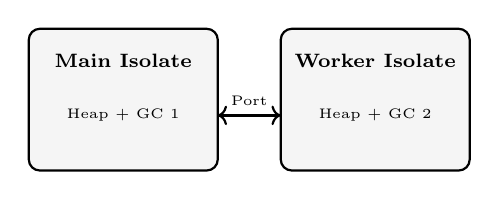
\begin{tikzpicture}
        \draw[thick, rounded corners, fill=gray!8] (0,0) rectangle (2.4,1.8);
        \node[font=\bfseries\scriptsize] at (1.2,1.4) {Main Isolate};
        \node[font=\tiny] at (1.2,0.7) {Heap + GC 1};

        \draw[thick, rounded corners, fill=gray!8] (3.2,0) rectangle (5.6,1.8);
        \node[font=\bfseries\scriptsize] at (4.4,1.4) {Worker Isolate};
        \node[font=\tiny] at (4.4,0.7) {Heap + GC 2};

        \draw[<->, thick] (2.4,0.7) -- (3.2,0.7) node[midway, above, font=\tiny] {Port};
      \end{tikzpicture}
    \end{column}
  \end{columns}
\end{frame}

% ------------------------------------------------------------------------------
% ------------------------------------------------------------------------------
% SLIDE 7: CƠ CHẾ HOẠT ĐỘNG CHI TIẾT CỦA HÀM COMPUTE()
% ------------------------------------------------------------------------------
\begin{frame}{Cơ chế hoạt động của hàm \texttt{compute()}}
  \vspace{-0.15cm}
  \begin{columns}[c]
    \begin{column}{0.53\textwidth}
      \footnotesize
      \textbf{1. Bản chất: Short-lived Isolate (Dùng một lần)}
      \begin{itemize}
        \setlength{\itemsep}{1pt}
        \item Hàm tiện ích cao cấp của Flutter (\texttt{foundation.dart}).
        \item Mô hình \textbf{One-shot (Fire-and-forget)}: Tự động khởi sinh để giải quyết 1 tác vụ rồi tự hủy.
      \end{itemize}
      \vspace{0.1cm}
      \textbf{2. Chu trình 4 bước bên dưới (Under the hood):}
      \begin{itemize}
        \setlength{\itemsep}{1.5pt}
        \item \textbf{B1 (Spawn ngầm):} Khởi tạo Isolate phụ \& Heap độc lập với một cổng phản hồi đơn (\texttt{SingleResponsePort}).
        \item \textbf{B2 (Chuyển giao):} Truyền con trỏ hàm Top-level và dữ liệu đầu vào sang Isolate mới.
        \item \textbf{B3 (Thực thi):} Chạy trên nhân CPU riêng biệt $\rightarrow$ Main Thread hoàn toàn rảnh tay duy trì \textbf{60+ FPS}.
        \item \textbf{B4 (Exit \& Tự hủy):} Gọi \texttt{Isolate.exit()} trả kết quả về Main và \textbf{thu hồi 100\% RAM ngay lập tức}.
      \end{itemize}
      \vspace{0.1cm}
      \textbf{3. Quy tắc bắt buộc:}
      \begin{itemize}
        \setlength{\itemsep}{1pt}
        \item Hàm truyền vào phải là \textbf{Top-level} hoặc \textbf{static method} (không được bắt giữ closure hay con trỏ \texttt{this}).
      \end{itemize}
    \end{column}

    \begin{column}{0.45\textwidth}
      \centering
      \begin{tikzpicture}[scale=0.72, every node/.style={font=\scriptsize}]
        % Column Titles comfortably above boxes
        \node[font=\bfseries\scriptsize, align=center] at (-2.45, 4.05) {MAIN ISOLATE\\{\tiny (UI Thread)}};
        \node[font=\bfseries\scriptsize, align=center] at (2.45, 4.05) {WORKER ISOLATE\\{\tiny (Short-lived Heap)}};

        % Main Isolate Box
        \draw[thick, rounded corners, fill=gray!8] (-3.6, -0.5) rectangle (-1.3, 3.4);
        \node[draw, thick, fill=white, rounded corners, align=center, text width=1.8cm] (call) at (-2.45, 2.55) {\texttt{compute()}\\\tiny (gọi tác vụ)};
        \node[draw, dashed, fill=white, rounded corners, align=center, text width=1.8cm] (smooth) at (-2.45, 1.45) {\textbf{\tiny UI 60 FPS}\\ \tiny Không nghẽn!\\ \tiny Nhận chạm vuốt};
        \node[draw, thick, fill=white, rounded corners, align=center, text width=1.8cm] (result) at (-2.45, 0.35) {Nhận kết quả\\\tiny (\texttt{Future} xong)};

        % Worker Isolate Box (Dashed)
        \draw[thick, dashed, rounded corners, fill=gray!4] (1.3, -0.5) rectangle (3.6, 3.4);
        \node[draw, thick, fill=white, rounded corners, align=center, text width=1.8cm] (spawn) at (2.45, 2.55) {\textbf{1. Tự spawn}\\\tiny Heap riêng};
        \node[draw, thick, fill=white, rounded corners, align=center, text width=1.8cm] (exec) at (2.45, 1.45) {\textbf{2. Chạy hàm}\\\tiny CPU nhân 2};
        \node[draw, thick, fill=white, rounded corners, align=center, text width=1.8cm] (exit) at (2.45, 0.35) {\textbf{3. Tự hủy}\\\tiny \texttt{Isolate.exit()}};

        % Connectors with ample breathing space
        \draw[->, thick] (call) -- (spawn) node[midway, above, font=\tiny] {Truyền tham số};
        \draw[->, thick] (spawn) -- (exec);
        \draw[->, thick] (exec) -- (exit);
        \draw[->, thick] (exit) -- (result) node[midway, below, font=\tiny] {Trả kết quả};
      \end{tikzpicture}
    \end{column}
  \end{columns}
\end{frame}

% SLIDE 8: GIAO TIẾP QUA SENDPORT VÀ RECEIVEPORT
% ------------------------------------------------------------------------------
\begin{frame}{Cơ chế giao tiếp giữa các Isolate qua SendPort \& ReceivePort}
  \vspace{-0.15cm}
  \begin{columns}[c]
    \begin{column}{0.53\textwidth}
      \footnotesize
      \textbf{1. Bản chất cặp Port (Mô hình Actor trong Dart):}
      \begin{itemize}
        \setlength{\itemsep}{1.5pt}
        \item \textbf{\texttt{ReceivePort}:} Hộp thư nhận tin gắn với Isolate tạo ra nó. Hoạt động như một \texttt{Stream<dynamic>} bất đồng bộ, chỉ đọc.
        \item \textbf{\texttt{SendPort}:} Cổng gửi tin có thể truyền xuyên biên giới Isolate (Serializable). Cho phép mô hình Nhiều gửi -- Một nhận (Many-to-One).
      \end{itemize}
      \vspace{0.1cm}
      \textbf{2. Chu trình giao tiếp 4 bước (Handshake Protocol):}
      \begin{itemize}
        \setlength{\itemsep}{1.5pt}
        \item \textbf{B1 (Bắt tay):} Main tạo \texttt{ReceivePort}, gửi \texttt{sendPort} làm tham số khởi tạo qua lệnh \texttt{Isolate.spawn()}.
        \item \textbf{B2 (Báo tiến độ):} Worker tính toán nặng, định kỳ gửi bản tin \texttt{sendPort.send(\{'progress': x\})}.
        \item \textbf{B3 (Cập nhật UI):} Main dùng \texttt{await for} lắng nghe Stream $\rightarrow$ gọi \texttt{setState()} giữ vững \textbf{60+ FPS}.
        \item \textbf{B4 (Dọn dẹp):} Nhận tin \texttt{done} $\rightarrow$ gọi \texttt{rp.close()} và \texttt{iso.kill()} để \textbf{triệt tiêu nguy cơ rò rỉ RAM}.
      \end{itemize}
      \vspace{0.1cm}
      \textbf{3. Nguyên lý cốt lõi:} Không chia sẻ bộ nhớ (No Shared Memory) $\rightarrow$ \textbf{Triệt tiêu 100\% Race Condition / Deadlock}.
    \end{column}

    \begin{column}{0.45\textwidth}
      \centering
      \begin{tikzpicture}[scale=0.72, every node/.style={font=\scriptsize}]
        % Column Titles comfortably above boxes
        \node[font=\bfseries\scriptsize, align=center] at (-2.55, 3.95) {MAIN ISOLATE\\{\tiny (UI Thread)}};
        \node[font=\bfseries\scriptsize, align=center] at (2.55, 3.95) {WORKER ISOLATE\\{\tiny (Background Heap)}};

        % Main Isolate Box
        \draw[thick, rounded corners, fill=gray!8] (-3.8, -0.45) rectangle (-1.3, 3.35);
        \node[draw, thick, fill=white, rounded corners, align=center, text width=1.65cm] (rp) at (-2.55, 2.55) 
          {\textbf{\texttt{ReceivePort}}\\\tiny (Mở Stream nhận)};
        \node[draw, dashed, fill=white, rounded corners, align=center, text width=1.65cm] (ui) at (-2.55, 1.45) 
          {\textbf{\tiny UI 60+ FPS}\\\tiny \texttt{await for} $\rightarrow$ State};
        \node[draw, thick, fill=white, rounded corners, align=center, text width=1.65cm] (kill) at (-2.55, 0.35) 
          {\textbf{\tiny B4: Dọn dẹp RAM}\\\tiny \texttt{close()} \& \texttt{kill()}};

        % Worker Isolate Box
        \draw[thick, rounded corners, fill=gray!4] (1.3, -0.45) rectangle (3.8, 3.35);
        \node[draw, thick, fill=white, rounded corners, align=center, text width=1.65cm] (sp) at (2.55, 2.55) 
          {\textbf{\texttt{SendPort}}\\\tiny (Cổng nhận từ B1)};
        \node[draw, thick, fill=white, rounded corners, align=center, text width=1.65cm] (calc) at (2.55, 1.45) 
          {\textbf{\tiny Xử lý nặng 132MB}\\\tiny Parse \& Lượng giác};
        \node[draw, thick, fill=white, rounded corners, align=center, text width=1.65cm] (done) at (2.55, 0.35) 
          {\textbf{\tiny B3: Gửi Done}\\\tiny \texttt{send(\{'done'\})}};

        % Connectors perfectly spanning the gap
        \draw[->, thick, dashed] (-1.3, 2.55) -- (1.3, 2.55) 
          node[midway, above, font=\tiny, align=center] {\textbf{1.} Gửi \texttt{sendPort}\\lúc spawn};
        \draw[<-, thick] (-1.3, 1.45) -- (1.3, 1.45) 
          node[midway, above, font=\tiny, align=center] {\textbf{2.} Báo tiến độ\\\texttt{send(progress)}};
        \draw[<-, thick] (-1.3, 0.35) -- (1.3, 0.35) 
          node[midway, above, font=\tiny, align=center] {\textbf{3.} Bắn kết quả\\hoàn tất};
      \end{tikzpicture}
    \end{column}
  \end{columns}
\end{frame}

% ------------------------------------------------------------------------------
% SLIDE 9: ĐẶT LÊN BÀN CÂN: HÀM COMPUTE() VS ISOLATE.SPAWN() (BẢNG MÀU XANH)
% ------------------------------------------------------------------------------
\begin{frame}{So sánh --- Hàm \texttt{compute()} vs \texttt{Isolate.spawn()}}
  \vspace{0.1cm}
  \centering
  \small
  \setlength{\tabcolsep}{4pt}
  \arrayrulecolor{white}
  \renewcommand{\arraystretch}{1.42}
  \begin{tabular}{|>{\raggedright\arraybackslash}p{2.6cm}|>{\raggedright\arraybackslash}p{5.1cm}|>{\raggedright\arraybackslash}p{5.3cm}|}
    \hline
    \rowcolor{TableHead}
    \centering\color{white}\textbf{Tiêu chí so sánh} & \centering\color{white}\textbf{Hàm \texttt{compute()} (Foundation)} & \centering\color{white}\textbf{\texttt{Isolate.spawn()} + Ports (Core)} \tabularnewline
    \hline
    \rowcolor{TableRowOdd}
    \textbf{Vòng đời\newline (Lifecycle)} & \textbf{Ngắn hạn (Short-lived):} Tự sinh ra, chạy 1 hàm duy nhất rồi tự hủy. & \textbf{Dài hạn (Long-lived):} Lập trình viên chủ động quản lý vòng đời và thời điểm hủy. \tabularnewline
    \hline
    \rowcolor{TableRowEven}
    \textbf{Khả năng báo tiến độ} & \textbf{Chỉ 1 lần:} Trả kết quả khi xong hoàn toàn (Fire-and-forget). & \textbf{Thời gian thực:} Truyền phát liên tục (Stream) các gói tin tiến độ (0\% $\rightarrow$ 100\%) qua SendPort. \tabularnewline
    \hline
    \rowcolor{TableRowOdd}
    \textbf{Độ phức tạp mã nguồn} & \textbf{Cực kỳ đơn giản:} Chỉ 1 dòng lệnh:\newline \texttt{await compute(task, args);} & \textbf{Trung bình:} Phải mở ReceivePort, lắng nghe Stream và gọi lệnh \texttt{kill()}. \tabularnewline
    \hline
    \rowcolor{TableRowEven}
    \textbf{Tình huống tối ưu} & Tác vụ nhanh gọn 1 lần: Parse JSON API, nén ảnh, giải mã dữ liệu. & Tác vụ kéo dài nhiều giây cần thanh tiến trình ProgressBar trực quan. \tabularnewline
    \hline
  \end{tabular}
\end{frame}

% ------------------------------------------------------------------------------
% SLIDE 10: THIẾT KẾ BÀI TOÁN THỰC NGHIỆM TRÊN WINDOWS DESKTOP
% ------------------------------------------------------------------------------
\begin{frame}{Thiết kế Bài toán Thực nghiệm trên Windows Desktop}
  \vspace{-0.25cm}
  \begin{columns}[c]
    \begin{column}{0.5\textwidth}
      \textbf{1. Thách thức với Vi xử lý mạnh (Intel Core i7-13th H):}
      \begin{itemize}
        \item Xung nhịp đơn nhân Turbo đạt tới $\mathbf{5.0\text{ GHz}}$.
        \item Nếu chỉ parse JSON 15MB thông thường: chỉ mất $\sim 180\text{ ms}$, giao diện chỉ giật nhẹ, không kịp thấy đơ!
      \end{itemize}
      \vspace{0.1cm}
      \textbf{2. Giải pháp Nhân tải Đa tầng:}
      \begin{itemize}
        \item \textbf{Dung lượng file lớn:} Tùy biến từ \textbf{16.5 MB} (60.000 bản ghi) đến \textbf{132.1 MB} (480.000 bản ghi cảm biến).
        \item \textbf{Tải tính toán FLOPS:} Lặp 25 lần tính toán lượng giác ($\sqrt{x}, \sin, \cos$) trên từng bản ghi.
        \item Tạo tải tính toán đủ lớn để làm nghẽn (freeze) Main Thread $\mathbf{3 - 8\text{ giây}}$.
      \end{itemize}
    \end{column}

    \begin{column}{0.48\textwidth}
      \textbf{3. Vì sao chọn Windows Desktop thay vì Web?}
      \begin{itemize}
        \item \textbf{Hạn chế Sandbox trên Web:} Môi trường trình duyệt cô lập bảo mật, không cho phép truy cập trực tiếp hệ thống tệp cục bộ (\texttt{dart:io}). 
        \item \textbf{Web không có Isolate thật sự:} Trình duyệt biên dịch sang JavaScript đơn luồng, không hỗ trợ \texttt{dart:isolate}. Hàm \texttt{compute()} trên Web tự fallback về Main Thread.
        \item \textbf{Windows Native Desktop:} Máy ảo Dart VM thực thi đa nhân x86\_64 thực thụ.
      \end{itemize}
    \end{column}
  \end{columns}
\end{frame}

% ------------------------------------------------------------------------------
% SLIDE 11: SƠ ĐỒ KIẾN TRÚC HỆ THỐNG (SYSTEM ARCHITECTURE DIAGRAM)
% ------------------------------------------------------------------------------
\begin{frame}{Sơ đồ Kiến trúc Hệ thống (System Architecture Diagram)}
  \vspace{-0.15cm}
  \centering
  \begin{tikzpicture}
    % Presentation Layer (Tầng Giao diện)
    \draw[thick, rounded corners, fill=gray!6] (-6.3,1.65) rectangle (6.3,3.15);
    \node[anchor=west, font=\bfseries\scriptsize] at (-6.0,2.85) {TẦNG GIAO DIỆN (Presentation Layer)};
    \node[draw, thick, fill=white, rounded corners, text width=5.2cm, align=center, font=\scriptsize] at (-3.1,2.2) 
      {\textbf{BenchmarkScreen}\\(Thanh trượt, Nút bấm điều khiển)};
    \node[draw, thick, fill=white, rounded corners, text width=5.2cm, align=center, font=\scriptsize] at (3.1,2.2) 
      {\textbf{FpsMonitorPanel}\\(Ticker đo FPS, Hoạt ảnh bánh răng)};

    % Service Layer (Tầng Nghiệp vụ & Đa luồng)
    \draw[thick, rounded corners, fill=gray!6] (-6.3,-0.35) rectangle (6.3,1.15);
    \node[anchor=west, font=\bfseries\scriptsize] at (-6.0,0.85) {TẦNG NGHIỆP VỤ \& ĐA LUỒNG (Service \& Isolate Layer)};
    \node[draw, thick, fill=white, rounded corners, text width=5.2cm, align=center, font=\scriptsize] at (-3.1,0.2) 
      {\textbf{JsonGeneratorService}\\(Sinh file JSON 132MB ngầm)};
    \node[draw, thick, fill=white, rounded corners, text width=5.2cm, align=center, font=\scriptsize] at (3.1,0.2) 
      {\textbf{IsolateWorkerService}\\(Điều phối Main, compute, spawn)};

    % Data Layer (Tầng Dữ liệu & Lưu trữ)
    \draw[thick, rounded corners, fill=gray!6] (-6.3,-2.35) rectangle (6.3,-0.85);
    \node[anchor=west, font=\bfseries\scriptsize] at (-6.0,-1.15) {TẦNG DỮ LIỆU \& LƯU TRỮ (Data \& File Storage Layer)};
    \node[draw, thick, fill=white, rounded corners, text width=5.2cm, align=center, font=\scriptsize] at (-3.1,-1.8) 
      {\textbf{SensorRecord Model}\\(Mô hình hóa dữ liệu \& vòng FLOPS)};
    \node[draw, thick, fill=white, rounded corners, text width=5.2cm, align=center, font=\scriptsize] at (3.1,-1.8) 
      {\textbf{large\_benchmark\_data.json}\\(Lưu trữ tập tin trên SSD/HDD)};

    % Connections between layers
    \draw[<->, thick] (-3.1,1.65) -- (-3.1,1.15);
    \draw[<->, thick] (3.1,1.65) -- (3.1,1.15);
    \draw[<->, thick] (-3.1,-0.35) -- (-3.1,-0.85);
    \draw[<->, thick] (3.1,-0.35) -- (3.1,-0.85);
  \end{tikzpicture}
\end{frame}

% ------------------------------------------------------------------------------
% SLIDE 12: SƠ ĐỒ LUỒNG DỮ LIỆU 1 --- MAIN THREAD VS HÀM COMPUTE()
% ------------------------------------------------------------------------------
\begin{frame}{Sơ đồ Luồng dữ liệu (Data Flow 1) --- Main Thread vs Hàm \texttt{compute()}}
  \begin{columns}[t]
    \begin{column}{0.48\textwidth}
      \textbf{Luồng 1: Chạy trực tiếp trên Main Thread}
      \vspace{0.15cm}
      \begin{itemize}
        \item Bấm nút $\rightarrow$ Gọi trực tiếp trên luồng chính.
        \item \textbf{Event Loop bị khóa cứng} suốt 4,800 ms.
        \item \textbf{Hậu quả:} Toàn bộ tương tác UI bị đóng băng, thao tác trên Slider bị vô hiệu hoá.
      \end{itemize}
      \vspace{0.2cm}
      \centering
      \begin{tikzpicture}[scale=0.68]
        \node[draw, thick] (btn) at (0,2.4) {\tiny Bấm nút Chạy};
        \node[draw, thick] (main) at (0,1.4) {\tiny Main Thread Parse 132MB};
        \node[draw, thick, dashed] (lock) at (0,0.4) {\textbf{\tiny EVENT LOOP BỊ KHÓA}};
        \node[draw, thick] (res) at (0,-0.6) {\tiny Hoàn tất $\rightarrow$ Mở lại UI};

        \draw[->, thick] (btn) -- (main);
        \draw[->, thick] (main) -- (lock);
        \draw[->, thick] (lock) -- (res);
      \end{tikzpicture}
    \end{column}

    \begin{column}{0.48\textwidth}
      \textbf{Luồng 2: Tách luồng bằng \texttt{compute()}}
      \vspace{0.15cm}
      \begin{itemize}
        \item Bấm nút $\rightarrow$ Gọi \texttt{compute(heavyParseTask, ...)}.
        \item Task chuyển sang \textbf{nhân CPU số 2} xử lý độc lập.
        \item \textbf{Kết quả:} Main Thread rảnh tay, \textbf{giữ vững 60+ FPS}!
      \end{itemize}
      \vspace{0.2cm}
      \centering
      \begin{tikzpicture}[scale=0.68]
        \node[draw, thick] (btn2) at (0,2.4) {\tiny Bấm nút Chạy};
        \node[draw, thick] (spawn) at (0,1.5) {\tiny Gọi \texttt{compute()}};
        \node[draw, thick] (iso) at (1.8,0.5) {\tiny Core 2 Parse};
        \node[draw, thick] (ui) at (-1.8,0.5) {\tiny Main 60 FPS};
        \node[draw, thick] (done) at (0,-0.5) {\tiny Nhận kết quả};

        \draw[->, thick] (btn2) -- (spawn);
        \draw[->, thick] (spawn) -| (iso);
        \draw[->, thick] (spawn) -| (ui);
        \draw[->, thick] (iso) |- (done);
      \end{tikzpicture}
    \end{column}
  \end{columns}
\end{frame}

% ------------------------------------------------------------------------------
% SLIDE 13: SƠ ĐỒ LUỒNG DỮ LIỆU 2 --- ISOLATE.SPAWN + SENDPORT / RECEIVEPORT
% ------------------------------------------------------------------------------
\begin{frame}{Sơ đồ Luồng dữ liệu (Data Flow 2) --- \texttt{Isolate.spawn} + Ports}
  \vspace{-0.2cm}
  \centering
  \begin{tikzpicture}
    % Lifelines
    \node[draw, thick, rounded corners, fill=gray!15, text width=3.2cm, align=center, font=\bfseries\scriptsize] (ui_h) at (-4.2, 2.7) {Main Thread (UI)};
    \node[draw, thick, rounded corners, fill=gray!15, text width=3.2cm, align=center, font=\bfseries\scriptsize] (iso_h) at (4.2, 2.7) {Worker Isolate};
    
    \draw[thick, dashed] (ui_h.south) -- (-4.2, -2.1);
    \draw[thick, dashed] (iso_h.south) -- (4.2, -2.1);

    % Step 1: Open ReceivePort
    \node[draw, thick, fill=white, font=\scriptsize, text width=2.6cm, align=center] at (-4.2, 2.0) {1. Mở ReceivePort};

    % Step 2: Spawn arrow
    \draw[->, thick] (-4.2, 1.4) -- (4.2, 1.0) node[midway, above, font=\scriptsize] {\texttt{Isolate.spawn(entryPoint, sendPort)}};

    % Step 3: Parse JSON on Isolate
    \node[draw, thick, fill=white, font=\scriptsize, text width=2.8cm, align=center] at (4.2, 0.4) {2. Parse JSON 132MB\\\& Tính toán FLOPS};

    % Step 4: Send progress
    \draw[<-, thick] (-4.2, -0.4) -- (4.2, 0.0) node[midway, above, font=\scriptsize] {Gửi tiến độ: \texttt{\{'progress': 0.25\}}};

    % Step 5: UI updates progress smoothly
    \node[draw, thick, fill=white, font=\scriptsize, text width=2.6cm, align=center] at (-4.2, -0.9) {UI cập nhật 25\%\\(Giữ vững 60 FPS)};

    % Step 6: Send complete
    \draw[<-, thick] (-4.2, -1.6) -- (4.2, -1.2) node[midway, above, font=\scriptsize] {Gửi hoàn tất: \texttt{\{'status':'done', 'ms':4210\}}};

    % Step 7: Close port
    \node[draw, thick, fill=white, font=\scriptsize, text width=2.6cm, align=center] at (-4.2, -2.1) {Đóng Port \& kill Isolate};
  \end{tikzpicture}
  \vspace{0.15cm}
  \begin{itemize}
    \item \textbf{Kỹ thuật Throttling:} Chia tổng số bước lặp $\div 20$, chỉ gửi đúng 20 bản tin để chống nghẽn hàng đợi tin nhắn (\textit{SendPort Flooding}).
  \end{itemize}
\end{frame}

% ------------------------------------------------------------------------------
% SLIDE 14: CẤU TRÚC THƯ MỤC CHUẨN & THUẬT TOÁN ĐO FPS (TICKER)
% ------------------------------------------------------------------------------
\begin{frame}{Cấu trúc thư mục chuẩn \& Thuật toán đo FPS (Ticker)}
  \vspace{-0.2cm}
  \begin{columns}[t]
    \begin{column}{0.48\textwidth}
      \textbf{Cấu trúc thư mục Clean Architecture:}\\[0.15cm]
      \footnotesize
      \begin{itemize}
        \setlength{\itemsep}{3.5pt}
        \item \textbf{lib/main.dart}:\newline Khởi tạo \& khởi chạy ứng dụng.
        \item \textbf{lib/models/sensor\_record.dart}:\newline Định nghĩa bản ghi và vòng lặp FLOPS.
        \item \textbf{lib/services/json\_generator\_service.dart}:\newline Sinh file JSON ngầm bằng StringBuffer.
        \item \textbf{lib/services/isolate\_worker\_service.dart}:\newline Điều phối 3 chế độ chạy Isolate.
        \item \textbf{lib/widgets/fps\_monitor\_panel.dart}:\newline Bộ đo FPS thời gian thực và biểu đồ cột.
        \item \textbf{lib/screens/benchmark\_screen.dart}:\newline Màn hình điều khiển và bảng kết quả.
      \end{itemize}
    \end{column}

    \begin{column}{0.48\textwidth}
      \textbf{Thuật toán đo FPS \& Bắt nghẽn UI:}\\[0.15cm]
      \footnotesize
      \begin{itemize}
        \setlength{\itemsep}{3pt}
        \item \textbf{Ticker gắn Vsync:} Lắng nghe từng chu kỳ quét màn hình từ phần cứng.
        \item \textbf{Đo FPS mỗi 250ms:}
        \vspace{-0.15cm}
        \[
          \text{FPS} = \left(\frac{\text{frameCount} \times 1000}{\Delta t_{\text{ms}}}\right).\text{clamp}(0, 240)
        \]
        \vspace{-0.15cm}
        \item \textbf{Thuật toán phát hiện nghẽn UI:}
        \vspace{0.08cm}
        \begin{tikzpicture}
          \node[draw=gray!35, fill=gray!8, rounded corners, text width=5.2cm, font=\scriptsize\ttfamily, inner sep=4.5pt] {
            if (gapMs > 250) \{\\
            \hspace*{1.0em}\_freezeMs = gapMs; \_currentFps = 0;\\
            \hspace*{1.0em}\textcolor{gray}{\textit{// Ghi nhận số ms đơ \& cập nhật UI}}\\
            \}
          };
        \end{tikzpicture}
      \end{itemize}
    \end{column}
  \end{columns}
\end{frame}

% ------------------------------------------------------------------------------
% SLIDE 15: XỬ LÝ NGOẠI LỆ CHẶT CHẼ & QUẢN LÝ BỘ NHỚ
% ------------------------------------------------------------------------------
\begin{frame}{Xử lý Ngoại lệ Đa Luồng \& Quản lý Tài Nguyên Bộ nhớ}
  \begin{columns}[t]
    \begin{column}{0.48\textwidth}
      \textbf{1. Bắt lỗi an toàn qua ranh giới Port:}
      \begin{itemize}
        \item Bọc toàn bộ logic Worker Isolate trong \texttt{try / catch}.
        \item Nếu xảy ra lỗi: Gửi gói tin \texttt{\{'type':'error'\}} về Main Thread.
        \item Main Thread đóng Port an toàn, ngăn chặn hiện tượng rò rỉ tài nguyên và treo luồng tiếp nhận (Hang UI).
      \end{itemize}
      \vspace{0.2cm}
      \textbf{2. Bắt buộc \texttt{await flush()} khi ghi file:}
      \begin{itemize}
        \item Bắt buộc có \texttt{await sink.flush()} và \texttt{await sink.close()} trước khi thoát Isolate để đảm bảo đẩy toàn bộ dữ liệu từ bộ đệm (buffer) ghi hoàn tất xuống ổ đĩa trước khi huỷ tiến trình.
      \end{itemize}
    \end{column}

    \begin{column}{0.48\textwidth}
      \textbf{3. Giải phóng tài nguyên chống rò rỉ RAM:}
      \begin{itemize}
        \item Khi hoàn tất hoặc gặp lỗi, lập tức gọi:
        \begin{itemize}
          \item \texttt{receivePort.close();} $\rightarrow$ Đóng Stream.
          \item \texttt{workerIsolate.kill();} $\rightarrow$ Tiêu hủy Isolate tức thì, giải phóng Heap về hệ điều hành.
        \end{itemize}
      \end{itemize}
      \vspace{0.2cm}
      \textbf{4. Ngăn chặn Compiler tối ưu hóa:}
      \begin{itemize}
        \item Sử dụng biến tích luỹ kiểm tra điều kiện ( \texttt{if (acc == 123456789.987)}) nhằm đảm bảo trình biên dịch không được bỏ qua vòng lặp tính toán (\textit{Dead-code elimination}).
      \end{itemize}
    \end{column}
  \end{columns}
\end{frame}

% ------------------------------------------------------------------------------
% SLIDE 16: KẾT QUẢ THỰC NGHIỆM ĐỐI CHIẾU THÔNG SỐ (CHUẨN BẢNG MÀU XANH)
% ------------------------------------------------------------------------------
\begin{frame}{Kết quả Thực nghiệm \& Bảng đối chiếu Thông số}
  \vspace{-0.2cm}
  \centering
  \small
  \setlength{\tabcolsep}{2.8pt}
  \arrayrulecolor{white}
  \renewcommand{\arraystretch}{1.2}
  \begin{tabular}{|>{\raggedright\arraybackslash}p{3.45cm}|c|c|c|}
    \hline
    \rowcolor{TableHead}
    \centering\color{white}\textbf{Chỉ số Đánh giá} & \color{white}\textbf{Main Thread} & \color{white}\textbf{Hàm \texttt{compute()}} & \color{white}\textbf{\texttt{Isolate.spawn()} + Ports} \\
    \hline
    \rowcolor{TableRowOdd}
    \textbf{Chỉ số FPS trung bình} & \textbf{0 FPS} (Đơ cứng) & \textbf{60+ FPS} (Mượt mà) & \textbf{60+ FPS} (Mượt mà) \\
    \hline
    \rowcolor{TableRowEven}
    \textbf{Thời gian đơ UI (Freeze)} & \textbf{13,174 ms} & \textbf{0 ms} & \textbf{0 ms} \\
    \hline
    \rowcolor{TableRowOdd}
    \textbf{Hoạt ảnh Bánh răng} & Đứng hình hoàn toàn & Xoay đều liên tục & Xoay đều liên tục \\
    \hline
    \rowcolor{TableRowEven}
    \textbf{Thanh trượt Test Slider} & Bị khóa cứng & Kéo thả mượt mà & Kéo thả mượt mà \\
    \hline
    \rowcolor{TableRowOdd}
    \textbf{Cập nhật \mbox{Progress Bar}} & Không thể cập nhật & Nhảy thẳng 100\% & Tịnh tiến 0\% $\rightarrow$ 100\% \\
    \hline
    \rowcolor{TableRowEven}
    \textbf{Thời gian thực thi} & 13,174 ms & 13,653 ms & 13,590 ms \\
    \hline
  \end{tabular}
  \vspace{0.3cm}
  \begin{itemize}
    \item \textbf{Đánh giá:} Dữ liệu ở mức tải 8x (480.000 bản ghi -- 132.1 MB) chứng minh rõ rệt: Hai giải pháp Isolate giúp giải phóng hoàn toàn Main Thread, duy trì giao diện mượt mà 60 FPS.
  \end{itemize}
\end{frame}

% ------------------------------------------------------------------------------
% SLIDE 17: MINH CHỨNG THỰC NGHIỆM GIAO DIỆN ỨNG DỤNG THỰC TẾ
% ------------------------------------------------------------------------------
\begin{frame}{Minh chứng Thực nghiệm: Giao diện Ứng dụng Thực tế}
  \vspace{0.05cm}
  \textbf{Giao diện ứng dụng Isolate FPS Benchmark \& Bộ đo khung hình thời gian thực trên Windows:}
  \par\vspace{0.12cm}
  \centering
  \fboxsep=0pt\fboxrule=0.6pt%
  \fbox{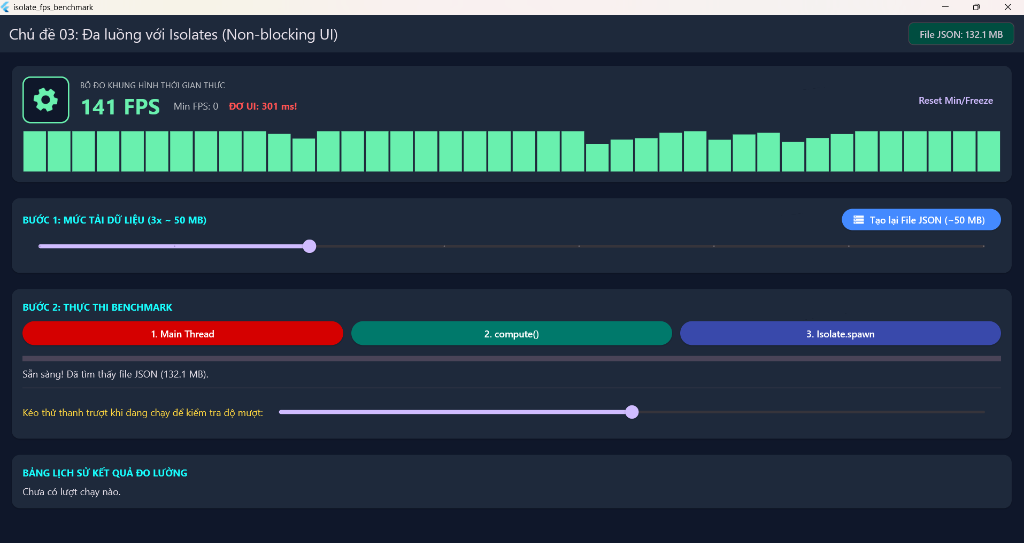
\includegraphics[width=0.98\textwidth,height=0.72\textheight,keepaspectratio]{app_benchmark_screen.png}}
\end{frame}

% ------------------------------------------------------------------------------
% SLIDE 18: KỊCH BẢN THỰC NGHIỆM LIVE DEMO TRỰC TIẾP
% ------------------------------------------------------------------------------
\begin{frame}{Chuyển sang Live Demo thực tế trên ứng dụng Windows}
  \begin{columns}[c]
    \begin{column}{0.54\textwidth}
      \begin{enumerate}
        \item \textbf{Khởi tạo dữ liệu:} Sinh file JSON 132.1 MB ngầm trong Isolate (không đơ UI lúc chuẩn bị dữ liệu).
        \item \textbf{Kiểm chứng Main Thread:}
        \begin{itemize}
          \item Bấm chạy $\rightarrow$ Bánh răng lập tức đứng khựng.
          \item Kéo Test Slider $\rightarrow$ Bị khóa đơ hoàn toàn.
          \item Bộ đo phát hiện và hiện cột đỏ \textbf{0 FPS} trong một khoảng thời gian!
        \end{itemize}
        \item \textbf{Kiểm chứng \texttt{compute()}:} Bấm chạy $\rightarrow$ Bánh răng vẫn xoay mượt mà ở \textbf{60+ FPS}.
        \item \textbf{Kiểm chứng \texttt{Isolate.spawn()}:} Bấm chạy $\rightarrow$ Bánh răng vẫn xoay mượt mà ở \textbf{60+ FPS} và thanh tiến trình tăng dần 0\% $\rightarrow$ 100\% theo thời gian thực.
      \end{enumerate}
    \end{column}

    \begin{column}{0.44\textwidth}
      \centering
      \begin{tikzpicture}[scale=0.75]
        \draw[thick] (0,0) rectangle (5.0,3.0);
        \node[font=\bfseries] at (2.5,2.7) {\scriptsize BẢNG ĐIỀU KHIỂN WINDOWS};
        \draw[thick] (0.4,1.4) rectangle (1.4,2.3);
        \draw[thick] (0.9,1.85) circle (0.22);
        \draw[thick, fill=black] (0.9,1.85) circle (0.07);
        \foreach \a in {0,45,...,315} {
          \draw[thick] (0.9,1.85) ++(\a:0.18) -- ++(\a:0.12);
        }
        \node[anchor=west, font=\bfseries] at (1.6,2.0) {\large 60 FPS};
        \node[anchor=west] at (1.6,1.5) {\tiny Real-time Monitor};
        \foreach \x in {0.4,0.7,...,4.6} {
          \draw[fill=gray!80] (\x, 0.4) rectangle (\x+0.2, 1.0);
        }
      \end{tikzpicture}
      \par\vspace{0.3cm}
      {\scriptsize \textit{(Nhóm xin phép chuyển sang cửa sổ ứng dụng Windows để thực hiện Live Demo trực tiếp)}\par}
    \end{column}
  \end{columns}
\end{frame}

% ------------------------------------------------------------------------------
% SLIDE 18: GIẢI THÍCH CÁC ĐOẠN MÃ NGUỒN THEN CHỐT (KEY CODE)
% ------------------------------------------------------------------------------
\begin{frame}[fragile]{Giải thích các đoạn Mã nguồn Then chốt}
  \begin{columns}[t]
    \begin{column}{0.48\textwidth}
      \textbf{1. Chạy trên Main Thread (Đơ UI):}
\begin{lstlisting}
ParseBenchmarkResult runOnMainThread(...) {
  return heavyParseTask({
    'filePath': path,
    'intensity': intensity,
  });
}
\end{lstlisting}
      \vspace{0.1cm}
      \textbf{2. Chạy bằng compute() (Gọn nhẹ):}
\begin{lstlisting}
Future<ParseBenchmarkResult> runWithCompute(...) async {
  return await compute(heavyParseTask, {
    'filePath': path,
    'intensity': intensity,
  });
}
\end{lstlisting}
    \end{column}

    \begin{column}{0.48\textwidth}
      \textbf{3. Chạy bằng Isolate.spawn (Báo tiến độ):}
\begin{lstlisting}
ReceivePort receivePort = ReceivePort();
Isolate iso = await Isolate.spawn(
  spawnIsolateEntry, 
  {'sendPort': receivePort.sendPort, ...}
);

await for (var msg in receivePort) {
  if (msg['type'] == 'progress') {
    onProgress(msg['progress']);
  } else if (msg['type'] == 'done') {
    receivePort.close();
    iso.kill(priority: Isolate.immediate);
    return res;
  }
}
\end{lstlisting}
    \end{column}
  \end{columns}
\end{frame}
% ------------------------------------------------------------------------------
% SLIDE 19: TỔNG KẾT & 3 QUY TẮC VÀNG
% ------------------------------------------------------------------------------
\begin{frame}{Tổng kết \& 3 Quy tắc vàng khi sử dụng Isolate}
  \textbf{3 QUY TẮC VÀNG KHI LỰA CHỌN GIẢI PHÁP ĐA LUỒNG TRONG FLUTTER:}
  \vspace{0.2cm}
  \begin{enumerate}
    \item \textbf{Quy tắc 1 (I/O thông thường):}
    \newline Nếu chỉ là gọi HTTP API, đọc file nhỏ vài KB hoặc truy vấn SQLite $\rightarrow$ \textbf{Dùng \texttt{async / await}}, KHÔNG dùng Isolate vì chi phí khởi tạo luồng lớn hơn thời gian chạy!
    \vspace{0.15cm}
    \item \textbf{Quy tắc 2 (Tác vụ nặng chạy 1 lần):}
    \newline Nếu cần bóc tách JSON lớn từ mạng, nén ảnh, xử lý dữ liệu một lần $\rightarrow$ \textbf{Dùng hàm \texttt{compute()}} (gọn nhẹ 1 dòng lệnh, tự sinh tự hủy, an toàn bộ nhớ).
    \vspace{0.15cm}
    \item \textbf{Quy tắc 3 (Tác vụ nặng kéo dài cần báo tiến độ):}
    \newline Nếu tác vụ kéo dài nhiều giây cần cập nhật thanh tiến trình ProgressBar liên tục $\rightarrow$ \textbf{Dùng \texttt{Isolate.spawn()} kết hợp SendPort / ReceivePort}.
  \end{enumerate}
\end{frame}

% ------------------------------------------------------------------------------
% SLIDE 21: TÀI LIỆU THAM KHẢO (THEO ĐÚNG TEMPLATE)
% ------------------------------------------------------------------------------
\begin{frame}{Tài liệu tham khảo}
  \textbf{Tài liệu kỹ thuật chính thức \& Tài liệu tham khảo:}
  \vspace{0.3cm}
  \begin{enumerate}
    \item \textbf{Google Flutter Documentation (2026):} \textit{Concurrency and isolates in Dart}, Official Guides. \url{https://dart.dev/guides/language/concurrency}
    \vspace{0.15cm}
    \item \textbf{Dart VM Core Library:} Thư viện chuẩn \texttt{dart:isolate}, \texttt{dart:async}, và mã nguồn hàm \texttt{compute()} trong \texttt{package:flutter/foundation.dart}.
    \vspace{0.15cm}
    \item \textbf{Flutter Performance Guide:} \textit{Profiling Flutter apps and diagnosing dropped frames (Build, Layout, Paint)}, Flutter Architecture Overview.
    \vspace{0.15cm}
    \item \textbf{Kho lưu trữ mã nguồn Đồ án (GitHub):} Dự án mã nguồn mở \texttt{isolate\_fps\_benchmark} trên nền tảng Windows Desktop Native.\\
    \url{https://github.com/KhoaLe246205/cross-platform/tree/main/isolate}
  \end{enumerate}
\end{frame}

% ------------------------------------------------------------------------------
% SLIDE 22: LỜI CẢM ƠN & PHIÊN PHẢN BIỆN (Q&A)
% ------------------------------------------------------------------------------
\begin{frame}[plain]
  \centering
  \vspace{1.8cm}
  {\LARGE \textbf{XIN CHÂN THÀNH CẢM ƠN!}}\\[0.3cm]
  {\large \textbf{QUÝ THẦY VÀ CÁC BẠN ĐÃ LẮNG NGHE}}\\[1.0cm]
 
\end{frame}

\end{document}